\section{Numerical Experiments}
\red{Don't forget to trim figures and convert them to pdfs!}

\subsection{Convection-Diffusion(-Reaction)} \label{sec:cdvcdr}

In this section, we demonstrate the method derived in Section \ref{sec:deriv} for two models which differ in the physics included. We first describe the problem setup, and then present results from applying our approach.

%------------------------------------------------------------%
\subsection{Problem Setup} \label{sec:cdvcdrSetup}
%------------------------------------------------------------%

The high- and low-fidelity models are restricted to a rectangular domain $\Omega$, defined as $\Omega(x_1,x_2)=[0,5]\times[0,1]$, where $x_1$ and $x_2$ are the spatial coordinates. The high-fidelity model is a single-species convection-diffusion-reaction equation with a nonlinear reaction term, described by
\begin{equation}
k_d\nabla^2 u - \vec{V}\cdot\nabla u + k_ru^2= f(q),
\label{eq:cdvcdrHF}
\end{equation}
where the state $u$ is the species concentration, $f(q)$ is a forcing field described by the parameters, $k_d = 0.1$ is a diffusion coefficient and $k_r = -42.0$ is a reaction coefficient. The low-fidelity model
\begin{equation}
k_d\nabla^2 u - \vec{V}\cdot\nabla u = f(q)
\end{equation}
differs only in the removal of the reaction term. Both models share a common velocity field, described by $\vec{V}(x_1,x_2) = (2x_2(1-x_2),0)$. To form the mixed-fidelity models, we divide the domain into complementary subdomains, $\Omega_{HF}$ and $\Omega_{LF}$, where the high- and low-fidelity models are solved, respectively. The resulting mixed-fidelity models can be described by 
\begin{equation}
k_d\nabla^2 u - \vec{V}\cdot\nabla u + k^{MF}_ru^2= f(q),
\end{equation}
where $k^{MF}_r$ is a piecewise-constant reaction coefficient
\begin{equation}
k^{MF}_r=
\begin{cases}
-42.0 & \textrm{if }x\in\Omega_{HF} \\
0 & \textrm{if }x\in\Omega_{LF}.
\end{cases}
\end{equation}
Homogeneous Dirichlet boundary conditions are applied on the entire boundary of the domain.

We let the unknown parameters we wish to infer correspond to the forcing field, so that $f(q)=q$. Observations $d=(u(0.35,0.35),u(1.56,0.61),u(3.1,0.5))$ from three points in the domain are artificially generated by running the high-fidelity model on a finer mesh with a piecewise constant source term $f_{true}$
\begin{equation}
f_{true}(x_1,x_2)=
\begin{cases}
1.0 & \textrm{if }(x_1,x_2)\in[0.125,0.375]\times[0.125,0.375] \\
0.8 & \textrm{if }(x_1,x_2)\in[2.375,2.625]\times[0.375,0.625] \\
0 & \textrm{otherwise}.
\end{cases}
\end{equation}
The QoI we wish to calculate is the integral of the state,
\begin{equation}
I(q,u)=\int_{(x_1,x_2)\in \Omega_I} u \:\textrm{d}A,
\end{equation}
over a region $\Omega_I=[0.625,0.875]\times[0.375,0.625]$. The locations of the observations and the region $\Omega_I$ over which the QoI is calculated is shown in Figure \ref{fig:baseSetup}. Since the inverse problem is ill-posed, we use Tikhonov regularization \cite{EngHanNeu00}; the regularization term is $\frac{\beta}{2}\int_\Omega \|\nabla f(q)\|_2^2\:\textrm{d}A$, where $\beta=10^{-5}$ is a regularization coefficient.

\begin{figure}[h]
\centering
\includegraphics[width=0.8\textwidth]{baseSeries/setup_3_3.pdf}
\caption{Locations of the observations and the QoI region.}
\label{fig:baseSetup}
\end{figure}

For the numerical simulations, we use the \texttt{libMesh} library \cite{libMeshPaper}. The domain is discretized by a regular mesh of quadrilaterals, with 50 and 250 elements along the short and long boundaries, respectively, for a total of 12,500 elements. We implement the finite element method (FEM) for a continuous Galerkin formulation using a linear nodal basis, for a total of 76,806 degrees of freedom. The P\'{e}clet number never exceeds 0.1 in any part of the domain, so we do not require stabilization.

%------------------------------------------------------------%
\subsection{Adaptive Model Refinement} \label{sec:cdvcdrBaseRef} 
%------------------------------------------------------------%

Once the QoI error estimate is calculated using Equation (\ref{eq:finErrExp}), the error estimate is then localized to each element to give an element-wise decomposition of the error. As described in Algorithm \ref{alg:refSeries}, based on this element-wise decomposition, we increase the proportion of the domain in which the high-fidelity model is used until the estimated absolute relative error in the QoI is less than $1\%$. Figure \ref{fig:baseRef} shows the element-wise decomposition of the error estimate, as well as the subdomains where the low- and high-fidelity models are used, for the series of mixed-fidelity models thus generated. The true and estimated absolute relative errors in the QoI for these same mixed-fidelity models are shown in Figure \ref{fig:baseErr}.

It can be seen that in this case, while the error estimates are not exact due to the nonlinear reaction term in the high-fidelity model, the error estimates are fairly accurate. In addition, the QoI that would have been obtained from solving the inverse problem with the high-fidelity model can be replicated to within $1\%$ with a mixed-fidelity model where the high-fidelity model is used in only $10.5\%$ of the domain.

\begin{figure}[h!]
\centering
  \begin{subfigure}[b]{\textwidth}
  \centering
    \includegraphics[width=0.48\textwidth]{baseSeries/cd_cdr_LF_divvy.pdf}
    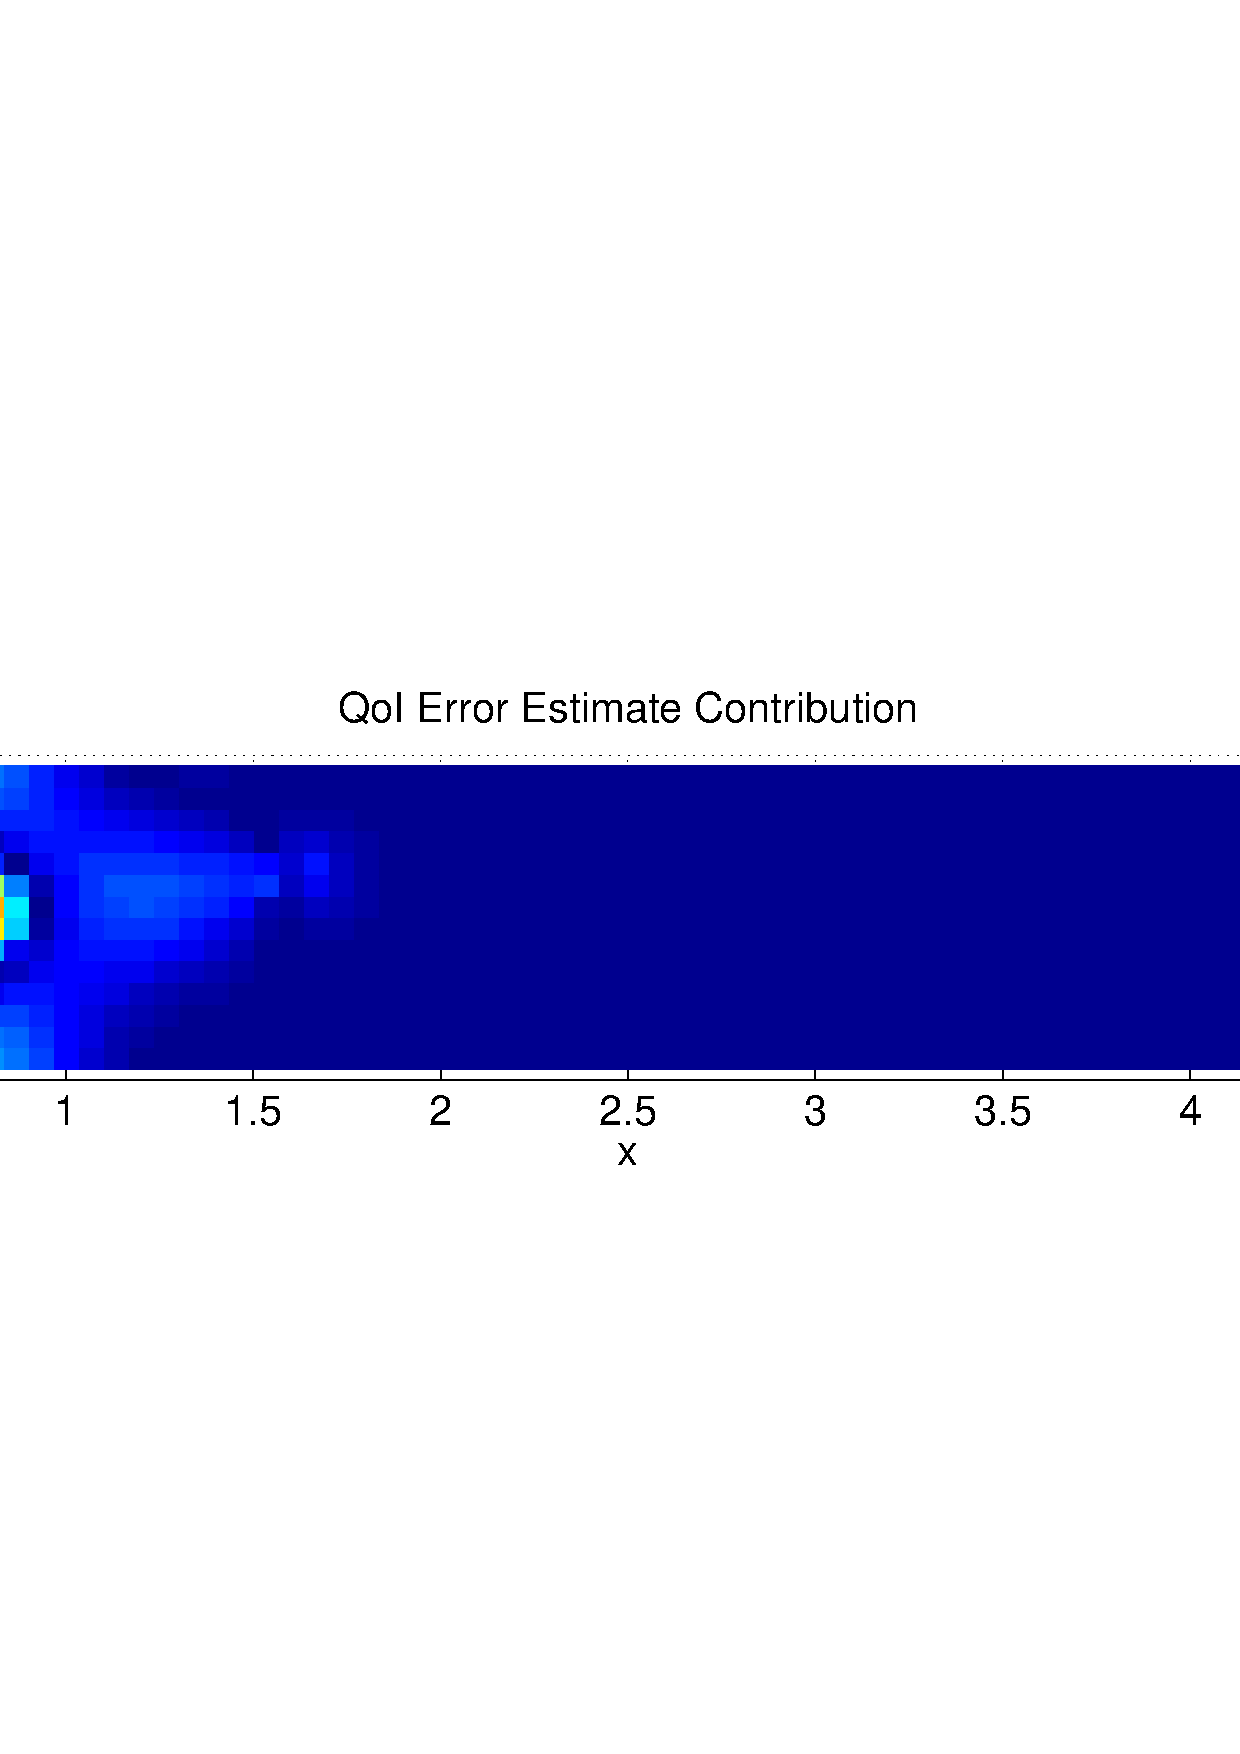
\includegraphics[width=0.49\textwidth]{baseSeries/err_breakdown_LF.png}
    \vspace{-0.5\baselineskip}
    \caption{MF$_0$ ($0\%$ HF)}
    \vspace{0.8\baselineskip}
  \end{subfigure}
	\begin{subfigure}[b]{\textwidth}
  \centering
    \includegraphics[width=0.48\textwidth]{baseSeries/cd_cdr_MF01_divvy.png}
    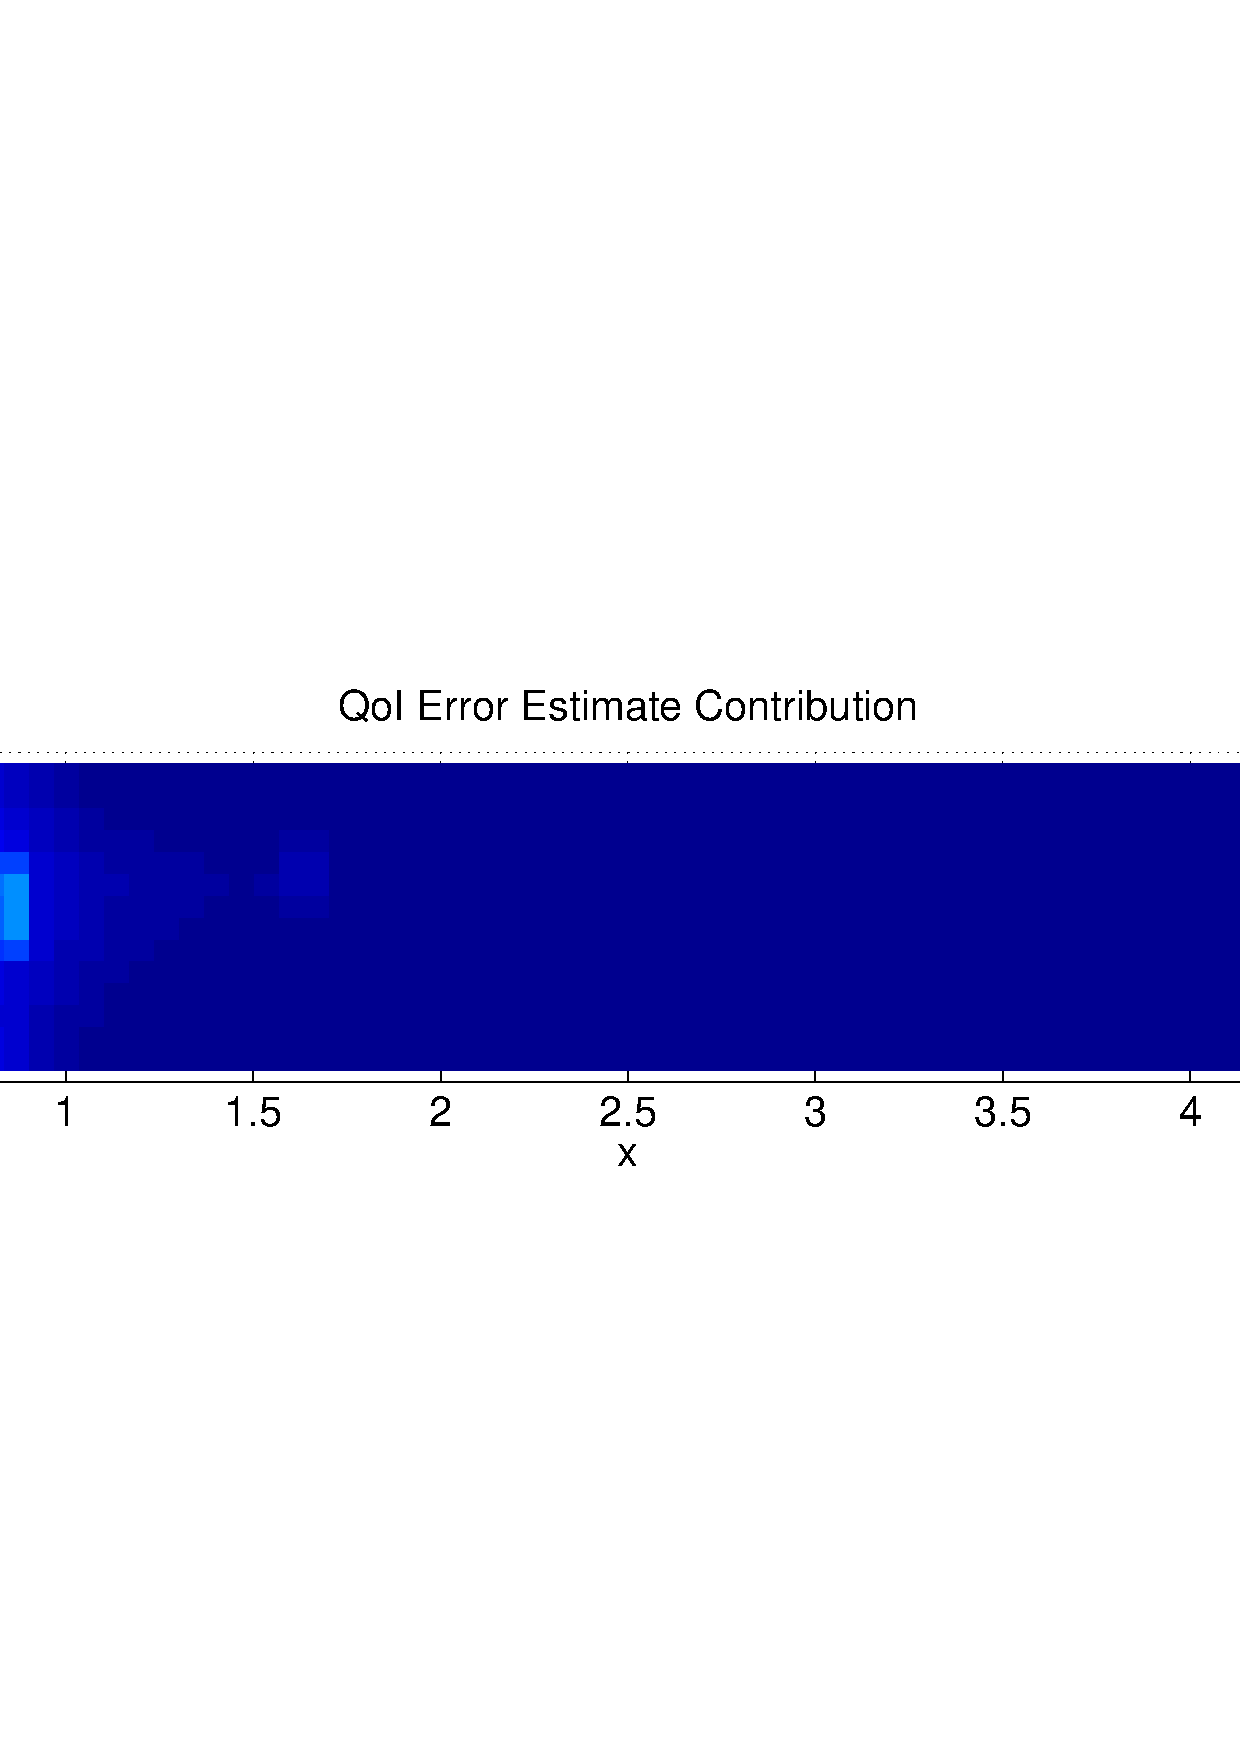
\includegraphics[width=0.49\textwidth]{baseSeries/err_breakdown_MF01.png}
    \vspace{-0.5\baselineskip}
    \caption{MF$_1$ ($5\%$ HF)}
    \vspace{0.8\baselineskip}
  \end{subfigure}
  \begin{subfigure}[b]{\textwidth}
  \centering
    \includegraphics[width=0.48\textwidth]{baseSeries/cd_cdr_MF02_divvy.png}
    \includegraphics[width=0.49\textwidth]{baseSeries/err_breakdown_MF02.png}
    \vspace{-0.5\baselineskip}
    \caption{MF$_2$ ($10\%$ HF)}
    \vspace{0.8\baselineskip}
  \end{subfigure}
\caption{Element-wise decomposition of error estimate (right) and domain division (left; low-fidelity convection-diffusion model used in red portion, high-fidelity convection-diffusion-reaction model used in blue portion) for mixed-fidelity models. Since linear nodal basis elements are used, elements in regions where the high-fidelity model is already being used do not contribute to the error estimate, except for some elements near the boundaries between low-fidelity and high-fidelity regions.}
\label{fig:baseRef}
\end{figure}

\begin{figure}[h]
\centering
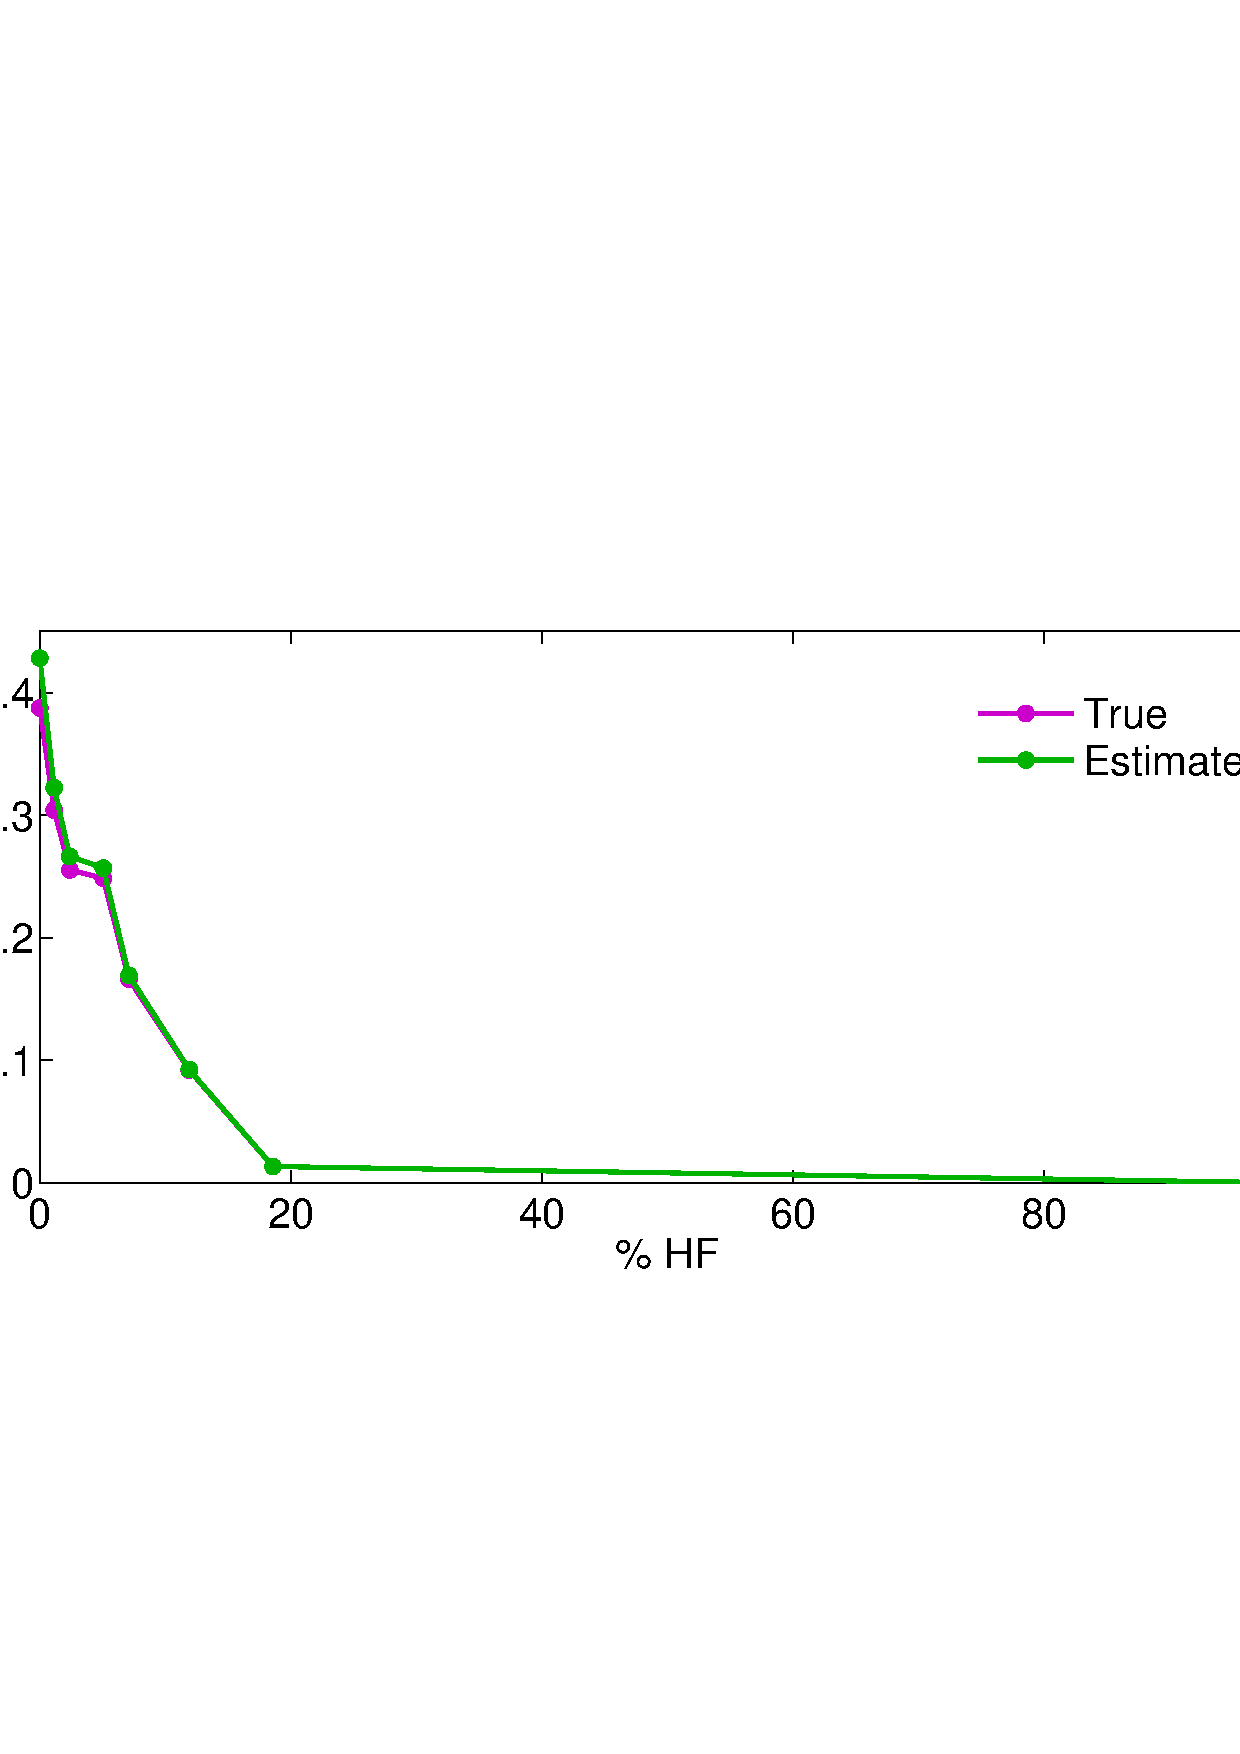
\includegraphics[width=0.8\textwidth]{baseSeries/err_est.pdf}
\caption{True and estimated absolute relative error in QoI, plotted as a function of the percentage area of the domain in which the high-fidelity convection-diffusion-reaction model is used.}
\label{fig:baseErr}
\end{figure}

\subsection{Constant vs Field Parameters}

\subsection{Cost Comparison}

\subsubsection{Simple Cost Analysis}

Consider a situation like that described in Section \ref{sec:cdvcdr}, where the state, adjoint, and parameter variables each have $N$ degrees of freedom. Suppose the low-fidelity model is linear, so that the cost of solving the inverse problem with the low-fidelity model (or with a mixed-fidelity model that is low-fidelity in most of the domain), is on the order of $(3N)^g$, where $g$ depends on the linear solver used. The cost for computing the auxiliary variables is also on the order of $(3N)^g$, and the cost for computing the supplementary adjoint is on the order of $(6N)^g$. Thus for $T$ iterations of the adaptive algorithm (where $T=1$ if one only calculates the error estimate relative to the low-fidelity model), the cost of using the adaptive algorithm is $T(2+2^g)(3N)^g$.

Suppose the inverse problem with the high-fidelity model is sufficiently nonlinear that a good initial guess is needed for convergence; one way to approach this is to use arclength continuation, a standard procedure in commercial nonlinear finite element programs.\footnote{According to Wikipedia...should see if we can confirm this elsewhere...} Letting $L_i$ represent the number of non-linear iterations required at each continuation step, the cost of solving the inverse problem with the high-fidelity model is $\sum_i L_i (3N)^g$. Assuming that the costs of both the high-fidelity inverse problem and adaptive algorithm are dominated by the cost of the linear solves, it is less costly to use Algorithm \ref{alg:refSeries} when $T<(2+2^g)^{-1}\sum_i L_i$. The bound on $T$ is strictest when $g=3$, as in the case where Gaussian elimination is used, giving $T<\frac{1}{10}\sum_i L_i$.

\subsubsection{Cost Comparison Example}

Here we consider the same problem as in Section \ref{sec:cdvcdr}, but with a reaction term $k_r=-616$ in the high-fidelity model. This reaction term is large enough that if the Newton solver will not converge with a zero initial guess. We first solve the inverse problem with the low-fidelity model ($k_r=0$), and then use the natural continuation approach, using the solution at one value of $k_r$ as the initial guess for the next.\footnote{NOT arclength continuation, which is more difficult to implement, though libMesh appears to have a class for such continuation, which we can use if this seems like a viable direction...}, We increase the reaction term in increments of $\Delta k_r=100$, and halve the increment each time the step is too large (Newton solver does not converge at the next $k_r$ value). From $k_r=0$ to $k_r=-616$, this results in 9 continuation steps being taken, with $\sum_i L_i=30$ linear solves of $N\times N$ systems required.

Since the low-fidelity model is linear in this case, solving for the primary and auxiliary variables takes one linear solve of an $N\times N$ system each. The error estimate is then used to choose $10\%$ of the domain in which to use the high-fidelity model. For this amount of refinement, the estimated relative error is $<1\%$; estimating the error requires five $N\times N$ linear solves for the primary variables and one linear $N\times N$ solve for the auxiliary variables. If adaption stops at this point, then the adaptive algorithm will have required $8+2(2^g)$ solves of $N\times N$ systems. For $g=3$ (Gaussian elimination), this amounts to 24 solves; with iterative methods where $g<3$, this number is smaller.

%does B+V's method for 'cheaply' getting auxiliary variables not really work when parameters are a field and not handful of scalars? does it even matter, since bulk of costs seem to be going to super-adjoint?
